%%%%%%%%%%%%%%%%%%%% 
%% Reminder: Bad At...
%%%%%%%%%%%%%%%%%%%% 
%\def\title{Two Big Problems}
%\begin{frame}{\title}
%
%\begin{center}
%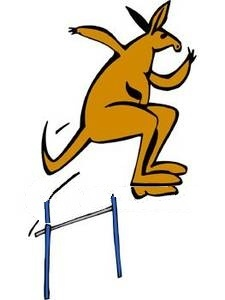
\includegraphics[height=3cm]{../img/hurdle.jpg}
%\end{center}
%
%\hh{1. People don't speak in atomic utterances}
%\vspace{2ex}
%
%\hh{2. Missing recall: the internet is incomplete} \\
%\end{frame}



%%%%%%%%%%%%%%%%%%% 
% Failed Search
%%%%%%%%%%%%%%%%%%% 
\input exampleSearchHeuristic.tex



%%%%%%%%%%%%%%%%%%% 
% Alignment
%%%%%%%%%%%%%%%%%%% 

\tikzset{
  arm angleA/.initial={0},
  arm angleB/.initial={0},
  arm lengthA/.initial={0mm},
  arm lengthB/.initial={0mm},
  arm length/.style={%
    arm lengthA=#1,
    arm lengthB=#1,
  },
  arm/.style={
    to path={%
      (\tikztostart) -- ++(\pgfkeysvalueof{/tikz/arm angleA}:\pgfkeysvalueof{/tikz/arm lengthA}) -- ($(\tikztotarget)+(\pgfkeysvalueof{/tikz/arm angleB}:\pgfkeysvalueof{/tikz/arm lengthB})$) -- (\tikztotarget)
    }
  },
}

%
% The slide
%
\def\title{Lexical Alignment Classifier}
\begin{frame}[fragile]{\title}
\newcommand{\hnode}[1]{|(#1)| \w{#1}}
\newcommand{\rnode}[2]{|(#1#2)| \w{\textcolor<2->{darkblue}{\textbf<2->{#1}}}\only<2->{\textcolor{white}{#2}}}
\newcommand{\bnode}[2]{|(#1#2)| \w{\textcolor<2->{darkblue}{\textcolor<6->{darkred}{\textbf<2->{#1}}}}\only<2->{\textcolor{white}{#2}}}

\begin{tikzpicture}
\matrix[column sep=-0.0em,row sep=1cm,matrix of nodes,row 2/.style={coordinate}] (m) {
% First sentence
\rnode{Forms}{$^p$} & \hnode{of} & \rnode{precipitation}{$^p$} & \bnode{include}{$^p$} & \rnode{rain}{$^p$} & \hnode{and} & \rnode{sleet}{$^p$} \\
\\
% Second sentence
\rnode{Rain}{$^c$} & \hnode{and} & \rnode{snow}{$^c$} & \hnode{are} & \rnode{forms}{$^c$} & \hnode{of} & \rnode{precipitation}{$^c$} \\
};
\only<3->{
\begin{scope}[every path/.style={line width=4pt,white,double=black},every to/.style={arm}, arm angleA=-90, arm angleB=90, arm length=5mm]
 \draw<3-3> (rain$^p$) to (Rain$^c$);
 \draw<3-3> (Forms$^p$) to (forms$^c$);
 \draw<3-3> (precipitation$^p$) to (precipitation$^c$);
 \draw<3-4> (sleet$^p$) to (snow$^c$);
 
 \draw<4-> [draw=green] (rain$^p$) to (Rain$^c$);
 \draw<4-> [draw=green] (Forms$^p$) to (forms$^c$);
 \draw<4-> [draw=green] (precipitation$^p$) to (precipitation$^c$);
 \draw<5-> [draw=red  ] (sleet$^p$) to (snow$^c$);
\end{scope}
}
\end{tikzpicture}

\pause
\pause
\pause
\vspace{2ex}

\hh{Features}
\begin{enumerate}
  \item Matching words
  \pause
  \item Mismatched words
  \pause
  \item Unmatched words in premise/consequent
\end{enumerate}
\pause
\vspace{1ex}
\hh{Competitive with Stanford RTE system (63\% on RTE3)}

\end{frame}



%%%%%%%%%%%%%%%%%%% 
% Lexical + Logic
%%%%%%%%%%%%%%%%%%% 
\def\title{Old Problem: Logic + Lexical Classifiers}
\begin{frame}{\title}
\begin{center}
\hh{FOL and lexical classifiers don't speak the same language} \\
\uncover<2->{\hh{...but natural logic does!}} \\
\vspace{2ex}
\only<1-1>{
\includegraphics[height=4cm]{../img/spy.png}}
\only<2->{
\includegraphics[height=4cm]{../img/speakwhale.jpg}}
\end{center}
\end{frame}

%%%%%%%%%%%%%%%%%%% 
% Big Picture
%%%%%%%%%%%%%%%%%%% 
\def\title{Big Picture}
\begin{frame}{\title}
\hh{Run our usual search}
\begin{enumerate}
\item If we find a premise, great!
\pause
\item If not, use lexical classifier as an \textit{evaluation function}
\end{enumerate}
\vspace{1ex}

\begin{center}
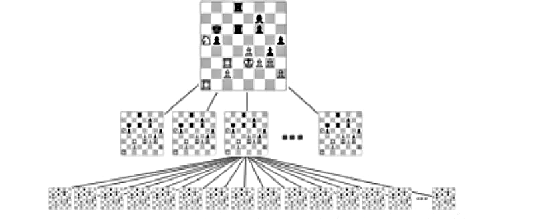
\includegraphics[height=3cm]{../img/chess.png}
\end{center}
\vspace{1ex}
\pause

\hh{Visit 1M nodes / second:} We have to be fast!
\end{frame}


%%%%%%%%%%%%%%%%%%% 
% Evaluation Function (Classifier)
%%%%%%%%%%%%%%%%%%% 
\def\title{Dissecting Our Classifier}
\begin{frame}{\title}
\hh{Anatomy of a Classifier}
\begin{itemize}
\item Features $f$ (matching / mismatched / unmatched words)
\item Weights $w$
\item Entailment pair $x$
\end{itemize}

\begin{center}
$p(\textrm{entail} \mid x) = \frac{1}{1 + \exp\left(-w^{\textrm{T}} f(x)\right)}$ \\
\pause
\vspace{3ex}
$p(\textrm{entail} \mid x)$ monotone w.r.t. $\left(w^{\textrm{T}} f(x)\right)$ \\
\end{center}
\pause
\vspace{1ex}

\begin{itemize}
\item Only need $w^{\textrm{T}} f(x)$ during search to compute $\max p(\textrm{entail} \mid x)$
\item $w^{\textrm{T}} f(x)$ is our evaluation function
\end{itemize}
\end{frame}

%%%%%%%%%%%%%%%%%%% 
% Evaluation Function (Search)
%%%%%%%%%%%%%%%%%%% 
\def\title{Incorporating our Evaluation Function}
\begin{frame}{\title}
\hh{Anatomy of a Search Step}
\begin{enumerate}
\item Mutate a word, or
\item Delete a word, or
\item Insert a word.
\end{enumerate}

\begin{center}
\hh{Each step updates a small number of features}
\end{center}

\begin{center}
\only<1-2>{
  \textcolor{darkgreen}{$w^{\textrm{T}}$} \textcolor{darkblue}{$f(x)$} = \textcolor{darkred}{$v$}
  \textcolor{white}{$x_i$} \\
}
\only<3->{
  \textcolor{darkred}{$v'$}
    = \textcolor{darkred}{$v$} 
    - \textcolor{darkgreen}{$w_i$} $\cdot$ \textcolor{darkblue}{$f_i$}
    + \textcolor{orange}{$w_i$} $\cdot$ \textcolor{orange}{$f_i$}
    \\
}
\vspace{1ex}
\only<1>{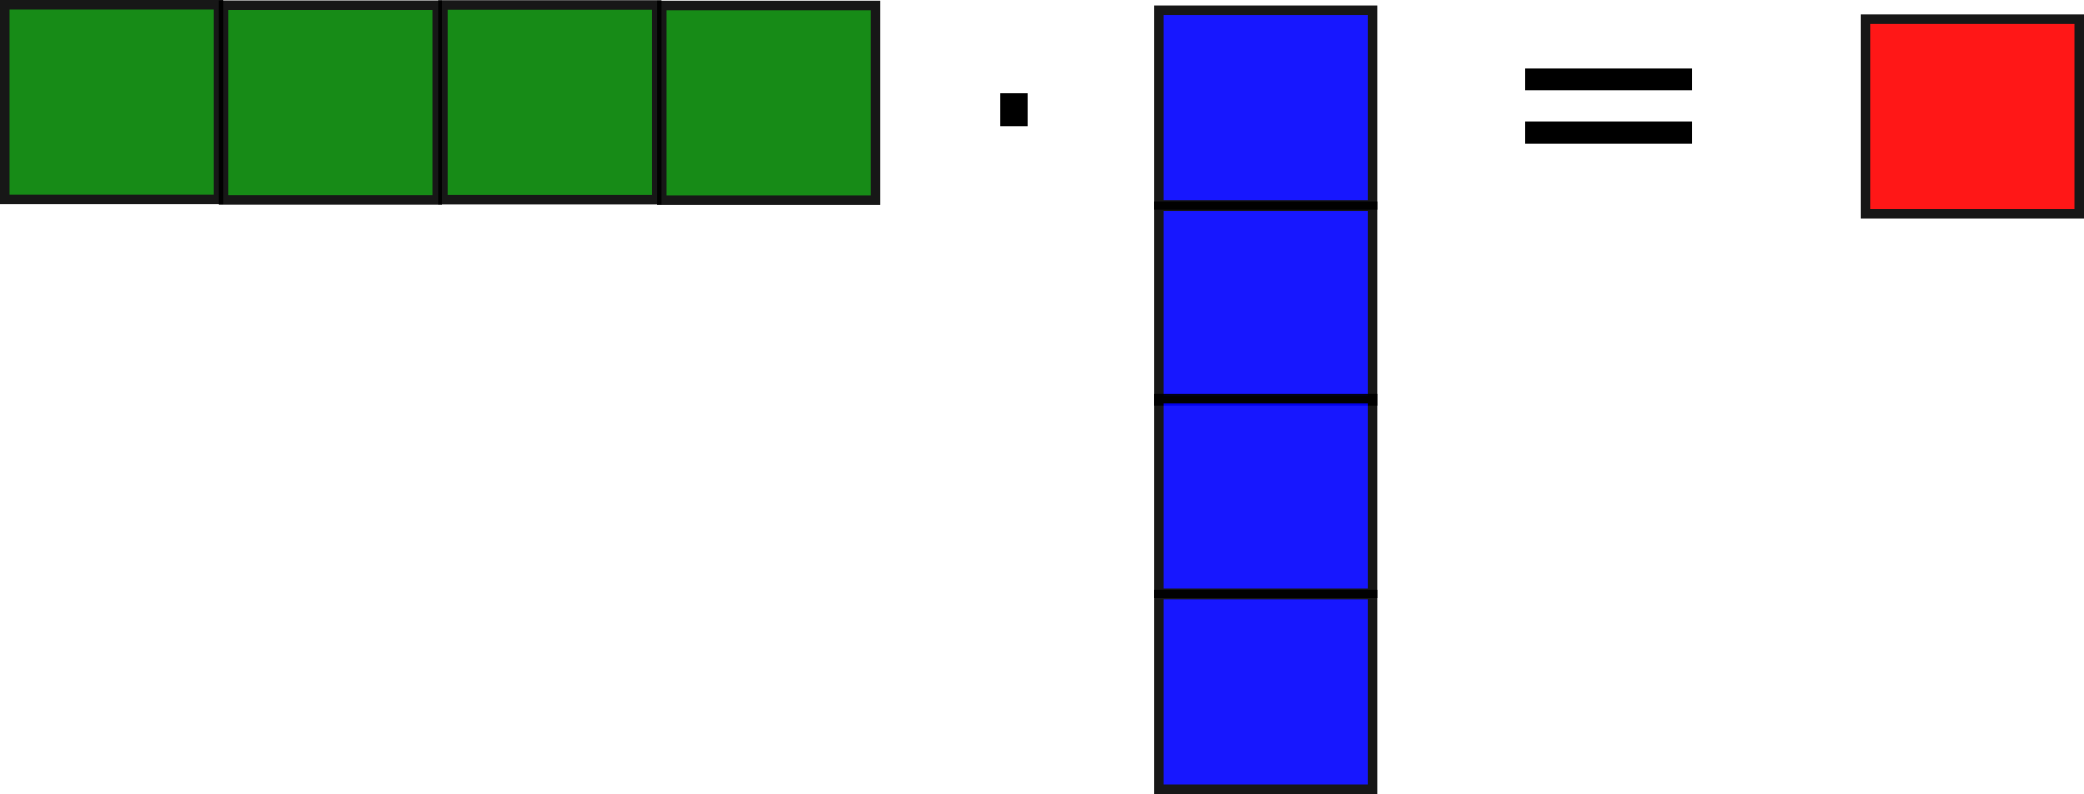
\includegraphics[height=2cm]{../img/dot.png}}
\only<2->{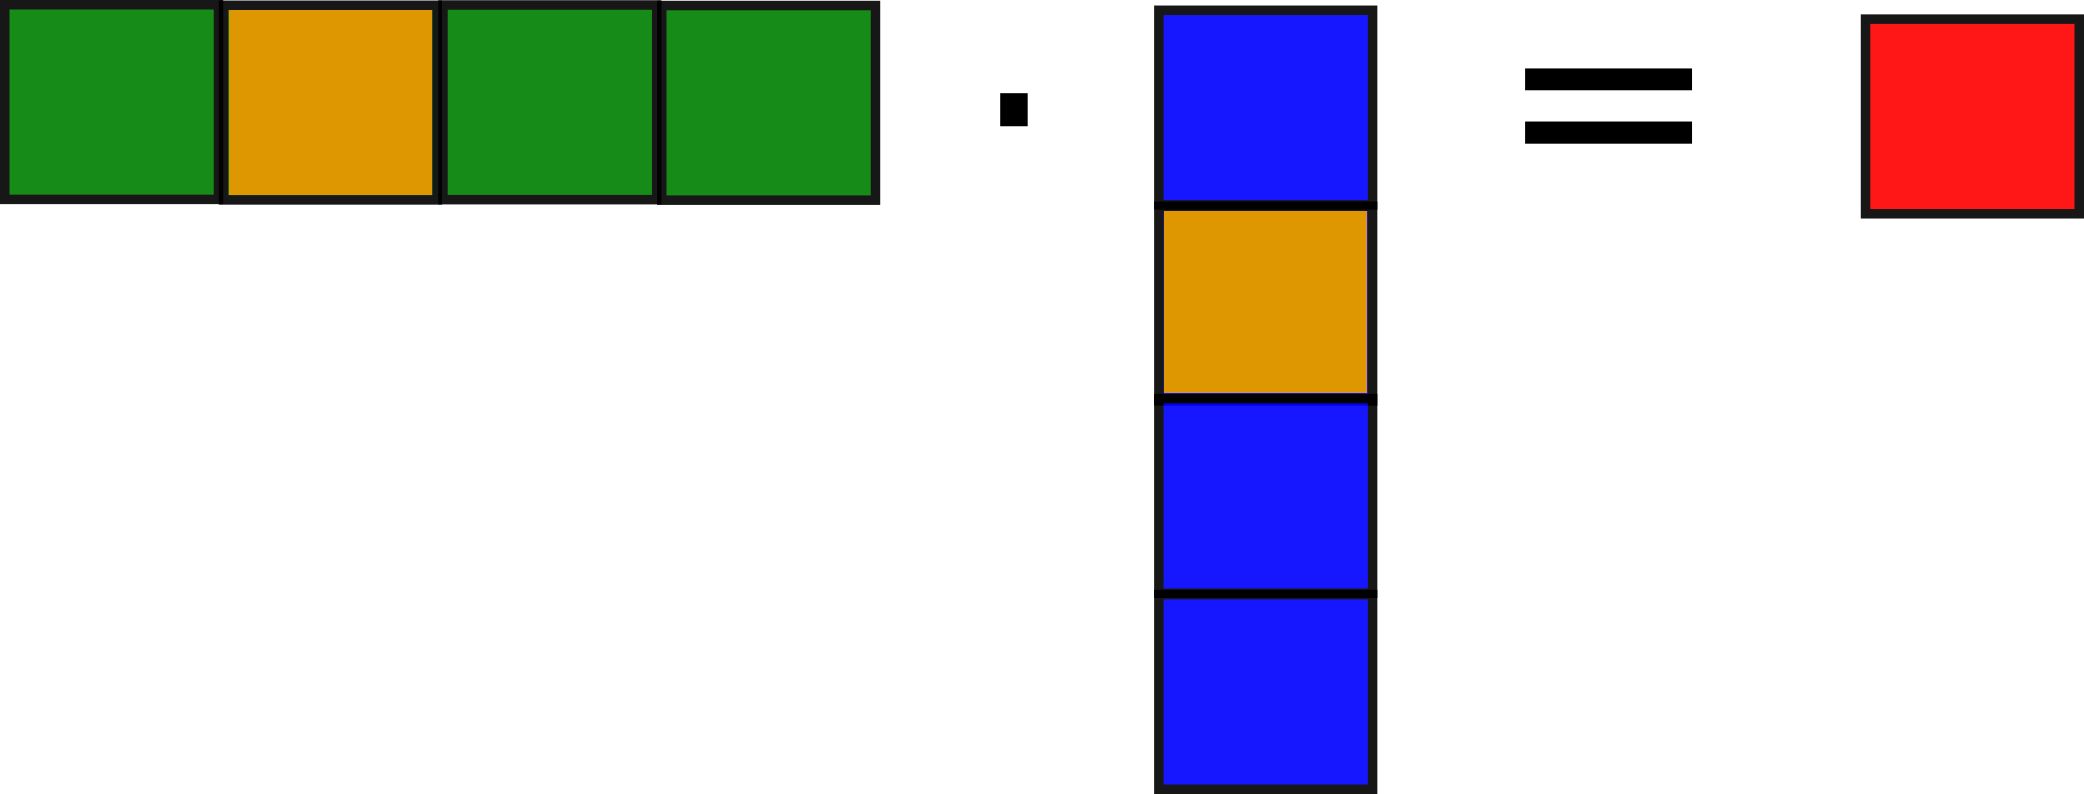
\includegraphics[height=2cm]{../img/dot-selected.png}}
\end{center}

\end{frame}


%%%%%%%%%%%%%%%%%%% 
% Synthesis
%%%%%%%%%%%%%%%%%%% 
\def\title{Why is this Important?}
\begin{frame}{\title}
\begin{center}

\includegraphics[height=2cm]{../img/efficient.png}
\end{center}

\hh{Faster Search $\Rightarrow$ Deeper Reasoning} 
\begin{itemize}
\item \textbf{Speed:} Around 1M search states visited per second
\item \textbf{Memory:} 32 byte search states
\end{itemize}
\vspace{2ex}

\hh{Speed:} Don't re-featurize at every timestep.
\vspace{2ex}

\hh{Memory:} Never store intermediate fact as String.
\end{frame}


%%%%%%%%%%%%%%%%%%% 
% Evaluation Function (Example)
%%%%%%%%%%%%%%%%%%% 


\newcommand{\hnode}[1]{|(#1)| \w{#1}}
\newcommand{\rnode}[2]{|(#1#2)| \w{\textcolor{darkblue}{\textbf{#1}}}\textcolor{white}{#2}}
\newcommand{\bnode}[2]{|(#1#2)| \w{\textcolor{darkblue}{\textcolor{darkred}{\textbf{#1}}}}\textcolor{white}{#2}}

\def\title{An Example Search}

%
% Frame 1
%
\begin{frame}[t,fragile]{\title}
\vspace{-5ex}
\begin{center}

\begin{tikzpicture}
\matrix[column sep=-0.0em,row sep=0.75cm,matrix of nodes,row 2/.style={coordinate}] (m) {
% First sentence
\rnode{Forms}{$^p$} & \hnode{of} & \rnode{precipitation}{$^p$} & \bnode{include}{$^p$} & \rnode{rain}{$^p$} & \hnode{and} & \rnode{sleet}{$^p$} \\
\\
% Second sentence
\rnode{Rain}{$^c$} & \hnode{and} & \rnode{snow}{$^c$} & \hnode{are} & \rnode{types}{$^c$} & \hnode{of} & \rnode{precipitation}{$^c$} \\
};
\begin{scope}[every path/.style={line width=4pt,white,double=black},every to/.style={arm}, arm angleA=-90, arm angleB=90, arm length=5mm]
 \draw [draw=green] (rain$^p$) to (Rain$^c$);
 \draw [draw=red] (Forms$^p$) to (types$^c$);
 \draw [draw=green] (precipitation$^p$) to (precipitation$^c$);
 \draw [draw=red  ] (sleet$^p$) to (snow$^c$);
\end{scope}
\end{tikzpicture}
\vspace{1ex}

\hh{Score $w^{\textrm{T}} f(x)$:} -0.5
\vspace{2ex}

\begin{tabular}{lrr}
\textbf{Feature} & \textbf{$w$} & \textbf{$f(x)$} \\
Matching words       &  2.0  & 2 \\
Mismatched words     & -1.0  & 2 \\
Unmatched premise    & -0.5  & 1 \\
Unmatched consequent & -0.75 & 0 \\
Bias                 & -2.0  & 1 
\end{tabular}
\end{center}
\end{frame}


%
% Frame 2
%
\begin{frame}[noframenumbering]{\title}
\exampleTreeLarge{ROOT \\ $~$}
                 {Rain and snow are types of precipitation}
                 {Rain and snow are \textbf{forms} of precipitation}
                 {Rain and snow are types of \textbf{weather}}
\end{frame}


%
% Frame 3
%
\begin{frame}[t,fragile,noframenumbering]{\title}
\vspace{-5ex}
\begin{center}

\begin{tikzpicture}
\matrix[column sep=-0.0em,row sep=0.75cm,matrix of nodes,row 2/.style={coordinate}] (m) {
% First sentence
\rnode{Forms}{$^p$} & \hnode{of} & \rnode{precipitation}{$^p$} & \bnode{include}{$^p$} & \rnode{rain}{$^p$} & \hnode{and} & \rnode{sleet}{$^p$} \\
\\
% Second sentence
\rnode{Rain}{$^c$} & \hnode{and} & \rnode{snow}{$^c$} & \hnode{are} & \rnode{forms}{$^c$} & \hnode{of} & \rnode{precipitation}{$^c$} \\
};
\begin{scope}[every path/.style={line width=4pt,white,double=black},every to/.style={arm}, arm angleA=-90, arm angleB=90, arm length=5mm]
 \draw [draw=green] (rain$^p$) to (Rain$^c$);
 \draw [draw=green] (Forms$^p$) to (forms$^c$);
 \draw [draw=green] (precipitation$^p$) to (precipitation$^c$);
 \draw [draw=red  ] (sleet$^p$) to (snow$^c$);
\end{scope}
\end{tikzpicture}
\vspace{1ex}

\hh{Score $w^{\textrm{T}} f(x)$:} 
  \only<1>{-0.5 + 2 $-$ -1}
  \only<2->{2.5}
\vspace{2ex}

\begin{tabular}{lrr}
\textbf{Feature} & \textbf{$w$} & \textbf{$f(x)$} \\
Matching words       &  2.0  & \textbf{3} \\
Mismatched words     & -1.0  & \textbf{1} \\
Unmatched premise    & -0.5  & 1 \\
Unmatched consequent & -0.75 & 0 \\
Bias                 & -2.0  & 1 
\end{tabular}
\end{center}
\end{frame}


%%
%% Frame 4
%%
%\begin{frame}[t,fragile,noframenumbering]{\title}
%\vspace{-5ex}
%\begin{center}
%
%\begin{tikzpicture}
%\matrix[column sep=-0.0em,row sep=0.75cm,matrix of nodes,row 2/.style={coordinate}] (m) {
%% First sentence
%\rnode{Forms}{$^p$} & \hnode{of} & \rnode{precipitation}{$^p$} & \bnode{include}{$^p$} & \rnode{rain}{$^p$} & \hnode{and} & \rnode{sleet}{$^p$} \\
%\\
%% Second sentence
%\rnode{Rain}{$^c$} & \hnode{} & \bnode{}{} & \hnode{are} & \rnode{forms}{$^c$} & \hnode{of} & \rnode{precipitation}{$^c$} \\
%};
%\begin{scope}[every path/.style={line width=4pt,white,double=black},every to/.style={arm}, arm angleA=-90, arm angleB=90, arm length=5mm]
% \draw [draw=green] (rain$^p$) to (Rain$^c$);
% \draw [draw=green] (Forms$^p$) to (forms$^c$);
% \draw [draw=green] (precipitation$^p$) to (precipitation$^c$);
%\end{scope}
%\end{tikzpicture}
%\vspace{1ex}
%
%\hh{Score $w^{\textrm{T}} f(x)$:} 
%  \only<1>{2.5 $-$ -1 $+$ -0.5}
%  \only<2->{2.0}
%\vspace{2ex}
%
%\begin{tabular}{lrr}
%\textbf{Feature} & \textbf{$w$} & \textbf{$f(x)$} \\
%Matching words       &  2.0  & 3 \\
%Mismatched words     & -1.0  & \textbf{0} \\
%Unmatched premise    & -0.5  & \textbf{2} \\
%Unmatched consequent & -0.75 & 0 \\
%Bias                 & -2.0  & 1 
%\end{tabular}
%\end{center}
%\end{frame}


%%%%%%%%%%%%%%%%%%% 
% Synthesis
%%%%%%%%%%%%%%%%%%% 
\def\title{The Full System}
%
% Frame 1
%
\begin{frame}{\title}
\begin{center}
\only<1>{\hh{Common Sense Reasoning}\textcolor{white}{p}}
\only<2>{\hh{$+$ Complex Premises}\textcolor{white}{p}}
\only<3>{\hh{$+$ Evaluation Function}\textcolor{white}{p}}

\begin{tikzpicture}

% horizontal axis
\draw[->] (0,0) -- (8,0) node[anchor=north] {Flexibility};
% vertical axis
\draw[->] (0,0) -- (0,4) node[anchor=east,rotate=90,yshift=1ex,xshift=5ex] {Coverage};

\node at (1.0,3.5)  {
\includegraphics[height=1cm]{../img/textrunner.jpg}};
\node at (7.0,1.0)  {
\includegraphics[height=1cm]{../img/pascal.png}};
\node at (3.5,2.5)  [visible on=<1>] {
\includegraphics[height=1cm]{../img/me.png}};
\node at (3.5,3.5)  [visible on=<2>] {
\includegraphics[height=1cm]{../img/me.png}};
\node at (7.0,3.5)  [visible on=<3>] {
\includegraphics[height=1cm]{../img/me.png}};

\end{tikzpicture}
\end{center}
\end{frame}

%
% Frame 2
%
\begin{frame}[noframenumbering]{\title}

\hh{Common Sense Facts}
\begin{itemize}
\item Natural logic inference as search
\item Soft relaxation of ``strict'' inference
\item 4x improvement in recall
\end{itemize}
\vspace{1ex}
\pause

\hh{Complex Premises}
\begin{itemize}
\item Split the premise into atomic clauses
\item Shorten each clause w/ natural logic
\item 3 F$_1$ improvement on knowledge base population
\end{itemize}
\vspace{1ex}
\pause

\hh{Evaluation Function}
\begin{itemize}
\item Use lexical classifier as evaluation function
\item Detect likely entailment / contradictions
\end{itemize}
\end{frame}

%%%%%%%%%%%%%%%%%%% 
% Results
%%%%%%%%%%%%%%%%%%% 
\def\bell{\raisebox{-2.5mm}{
\includegraphics[height=5mm]{../img/bell.png}}}
\def\whistle{\raisebox{-2.5mm}{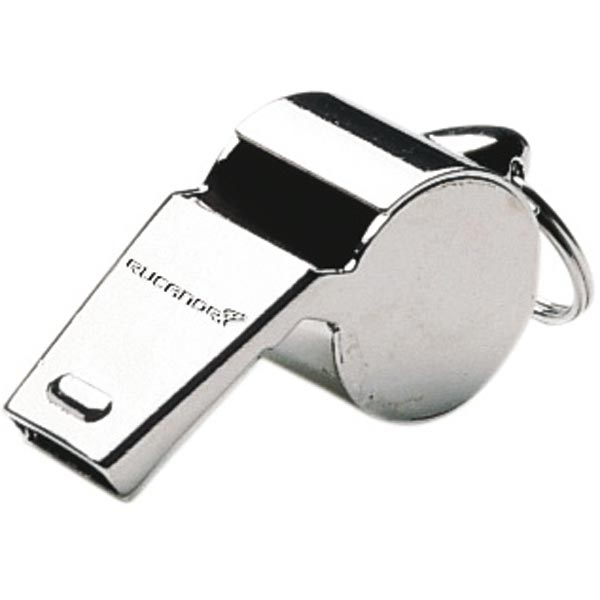
\includegraphics[height=5mm]{../img/whistle.jpg}}}
\def\title{Solving 4$^{th}$ Grade Science}

%
% Frame 1
%
\begin{frame}[t]{\title}
\hh{Multiple choice questions from real 4$^{th}$ grade science exams} \\
\vspace{2ex}
\pause

\textbf{Which activity is an example of a good health habit?}
\begin{enumerate}
\item[(A)] Watching television
\item[(B)] Smoking cigarettes
\item[(C)] Eating candy
\item[(D)] Exercising every day
\end{enumerate}
\vspace{2ex}
\pause

\textbf{In our corpus:}
\begin{itemize}
\item \w{Plasma TV's can display up to 16 million colors $\dots$ great for watching TV $\dots$ also make a good screen.}
\item \w{Not smoking or drinking alcohol is good for health, regardless of whether clothing is worn or not.}
\item \w{Eating candy for diner is an example of a poor health habit.}
\item \w{Healthy is exercising}
\end{itemize}

\end{frame}


%
% Frame 2
%
\begin{frame}[t,noframenumbering]{\title}
\footnotetext<.->{\cite{key:2015hixon-aristo}}

\hh{Multiple choice questions from real 4$^{th}$ grade science exams}
\begin{center}
\begin{tabular}{lcc}
\hline
\textbf{System}                & \textbf{Train}     & \textbf{Test} \\
\hline
\sc{Knowbot}                    & 45                & \only<4->{$-$} \\
\sc{Knowbot} (oracle)           & 57                & \only<4->{$-$} \\
\hline
\pause
IR Baseline                     & 49                & \only<4->{42} \\
This Thesis                     & 52                & \only<4->{51} \\
\hline
\pause
More Data + IR Baseline         & 62                & \only<4->{58} \\
More Data + This Thesis         & \textbf<3-4>{65}  & \only<4->{\textbf<4>{61}} \\
\hline
\pause
\pause
This Thesis + \bell + \whistle   & \textbf{74}        & \textbf{67} \\
\hline
\end{tabular}
\pause
\vspace{2ex}

\hh{We're able to pass 4$^{th}$ grade science!}

\end{center}
\end{frame}




